\documentclass[12pt]{article}
\usepackage{fullpage}
\usepackage{titlesec}
\usepackage{tikz}
\usetikzlibrary{automata, positioning}

\pagestyle{plain}
\titleformat{\subsection}[runin]
  {\normalfont\large\bfseries}{\thesubsection}{1em}{}

\title{Homework 2}
\author{Brooke Fugate, Michael O'Connor, Rohan Shah}
\date{}

\begin{document}
\maketitle

\section*{Problem B1}

\subsection*{(a)}
NFA with $2n+1$ states accepting $L_n$:
\newline
\begin{center}
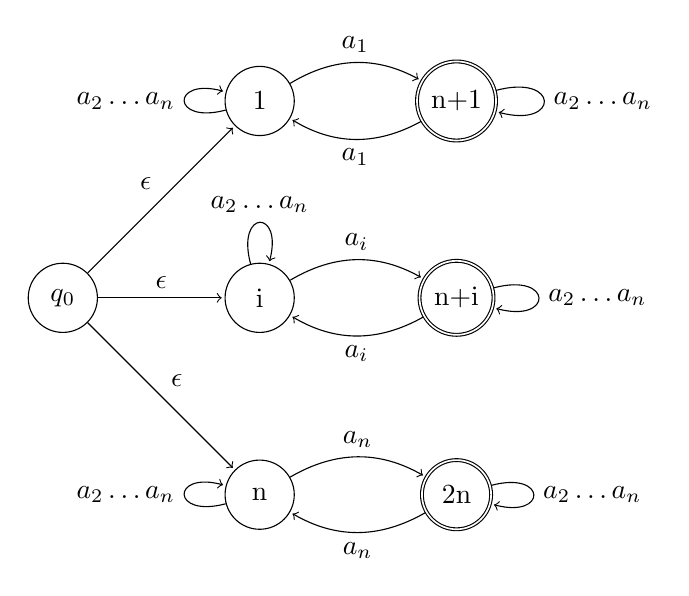
\begin{tikzpicture}[shorten >=1pt, node distance=2.5cm, on grid, auto]
  \node[state] (q0) {$q_0$};
  \node[state] (q2) [right=of q0] {i};
  \node[state] (q1) [above=of q2] {1};
  \node[state] (q3) [below=of q2] {n};
  \node[state, accepting] (q4) [right=of q1] {n+1};
  \node[state, accepting] (q5) [right=of q2] {n+i};
  \node[state, accepting] (q6) [right=of q3] {2n};
  \path[->]
  (q0) edge node {$\epsilon$} (q1)
       edge node {$\epsilon$} (q2)
       edge node {$\epsilon$} (q3)
  (q1) edge [loop left] node {$a_2 \dots a_n$} (q1)
  (q1) edge [bend left] node {$a_1$} (q4)
  (q4) edge [loop right] node {$a_2 \dots a_n$} (q4)
  (q4) edge [bend left] node {$a_1$} (q1)
  (q2) edge [loop above] node {$a_2 \dots a_n$} (q2)
  (q2) edge [bend left] node {$a_i$} (q5)
  (q5) edge [loop right] node {$a_2 \dots a_n$} (q5)
  (q5) edge [bend left] node {$a_i$} (q2)
  (q3) edge [loop left] node {$a_2 \dots a_n$} (q3)
  (q3) edge [bend left] node {$a_n$} (q6)
  (q6) edge [loop right] node {$a_2 \dots a_n$} (q6)
  (q6) edge [bend left] node {$a_n$} (q3)
  ;
\end{tikzpicture}
\end{center}
\subsection*{(b)}
  We can construct a DFA $D_i$ for each language $L^i_n$, where $L^i_n$ is the
  set of all strings over $\sum$ with an odd number of $a_i$, using two states
  as shown below. Since $L_n$ is the union of all such $L^i_n$, i.e.
  $L_n = L^1_n \cup \dots \cup L^n_n$ where $n$ is the number of symbols in the
  alphabet $\sum$, we can use the cross-product construction to combine each
  DFA $D_i$ and create a DFA $D$ that accepts the language $L_n$.
  The cross-product construction creates a DFA with $2^n$ states (since there
  are 2 states per DFA $D_i$ and thus the number of states in $D$ is doubled
  with each construction or n times). Thus there exists a DFA $D$ with $2^n$
  states that accepts the language $L_n$.
  \vspace{0.5cm}
  DFA $D_i$ that accepts the language $L^i_n$:
  \newline
  \begin{center}
  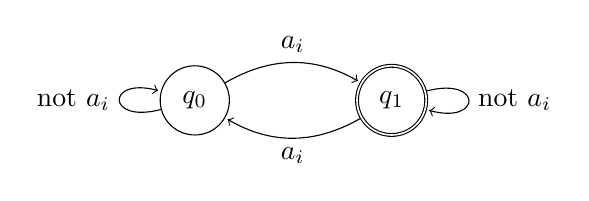
\begin{tikzpicture}[shorten >=1pt, node distance=2.5cm, on grid, auto]
    \node[state] (q0) {$q_0$};
    \node[state, accepting] (q1) [right=of q0] {$q_1$};
    \path[->]
    (q0) edge [bend left] node {$a_i$} (q1)
    (q0) edge [loop left] node {not $a_i$} (q0)
    (q1) edge [bend left] node {$a_i$} (q0)
    (q1) edge [loop right] node {not $a_i$} (q1)
    ;
  \end{tikzpicture}
  \end{center}

\subsection*{(c)}
\section*{Problem B2}
\subsection*{(a)}
\subsection*{(b)}
\section*{Problem B4}
\subsection*{(a)}
  Let $D = (Q, \sum, F, q_0, \delta)$ be the DFA that accepts the regular
  language L, i.e. $L(D) = L$. We can construct a DFA for the language
  $Pre(L)$ as $D_pre = (Q, \sum, F', q_0, \delta)$ where we define $F'$
  as follows.
\subsection*{(b)}
\subsection*{(c)}
\end{document}
